\chapter{Models and Evaluation}
\label{models}
This chapter expands on two of the main goals of the project: table detection in \ref{table_detection} and table classification in \ref{table_classification}. Each section reviews the models explored to meet these intents and the evaluation of the proposed solutions.

\section{Table detection}
\label{table_detection}
The task of table detection as addressed in this project is to detect and segment tables in newspapers pages. More formally, given an image of a scan of a newspaper page, the goal is to produce one or many segmentation masks that contain tables. Two image segmentation methods were used and compared to get a better idea of how best tackle the table detection problem. Even though these methods follow different image segmentation paradigms, they are both able to provide satisfactory solutions.

\subsection{dhSegment}
dhSegment \citep{ares_oliveira_dhsegment_2018} is a semantic image segmentation algorithm developed at the EPFL-DHLAB, which aims at providing a generic tool for historical document processing. Based on a U-Net architecture \citep{ronneberger_u-net_2015}, but incorporating a residual network as the encoder, it provides pixel-wise probability maps for each class to be detected. This model has already proven its effectiveness, especially in \citet{barman_combining_2021}, where it has shown encouraging results on newspaper pages. Note that all experiments were actually performed using dhSegment-torch\footnote{\url{https://github.com/dhlab-epfl/dhSegment-torch}}, a PyTorch reimplementation of the original model.

\paragraph{Semantic image segmentation}
We recall the definition of semantic image segmentation in the context of table detection. Semantic segmentation refers to the task of predicting the semantic class to which each pixel in an image belongs. In the table recognition use case, each pixel of the image must be defined as belonging either to the \textit{background} or to a \textit{table}. A segmentation mask for tables can then be produced. \\
One of the advantages of semantic segmentation is that the training material can be annotated at a coarse granularity: tables do not need to be individually annotated since they do not need to be individually detected. However, this makes the task of table classification very difficult, because it has to deal with a segmentation mask that may cover several tables from different classes, even when considering the different connected components (separate clusters of pixels) of the mask separately.

\paragraph{Model}
In this project, the architecture of dhSegment uses a ResNet-50 \citep{he_deep_2015} pre-trained on the ImageNet dataset \citep{deng_imagenet_2009} as its encoder. It uses the default implementation of dhSegment as described in the original paper, which limits the number of features channels in the expanding path to 512 for memory reasons.

\paragraph{Training}
The training hyper-parameters are detailed later for each experiment, as they vary slightly. However, what remains constant is the use of the mean intersection over union (mIoU) metric (see Section \ref{table_detection_evaluation}) to guide the training of the network.

\paragraph{Inference}
For the task of table detection, the network is asked to output two probability maps that indicate the likeliness each pixel is part of the \textit{background} or part of a \textit{table}. A prediction map is then created from these two probability maps, where each pixel is assigned to the most probable class. Finally, the connected components that represent less than 0.5\% of the page are removed, in agreement with the methodology proposed in \cite{barman_historical_2019}. In Figure \ref{inference_dhsegment}, a complete example is shown where the leftmost image corresponds to a ground truth, with tables annotated in a lighter colour; the middle image shows the probability map for the table class; and the rightmost image shows the final prediction. The spot on the left of the probability map is not part of the final prediction because the network has determined it as more likely to be part of the background. 

\begin{figure}
\centering
\begin{tabular}{ccc}
\subfloat[Ground truth]{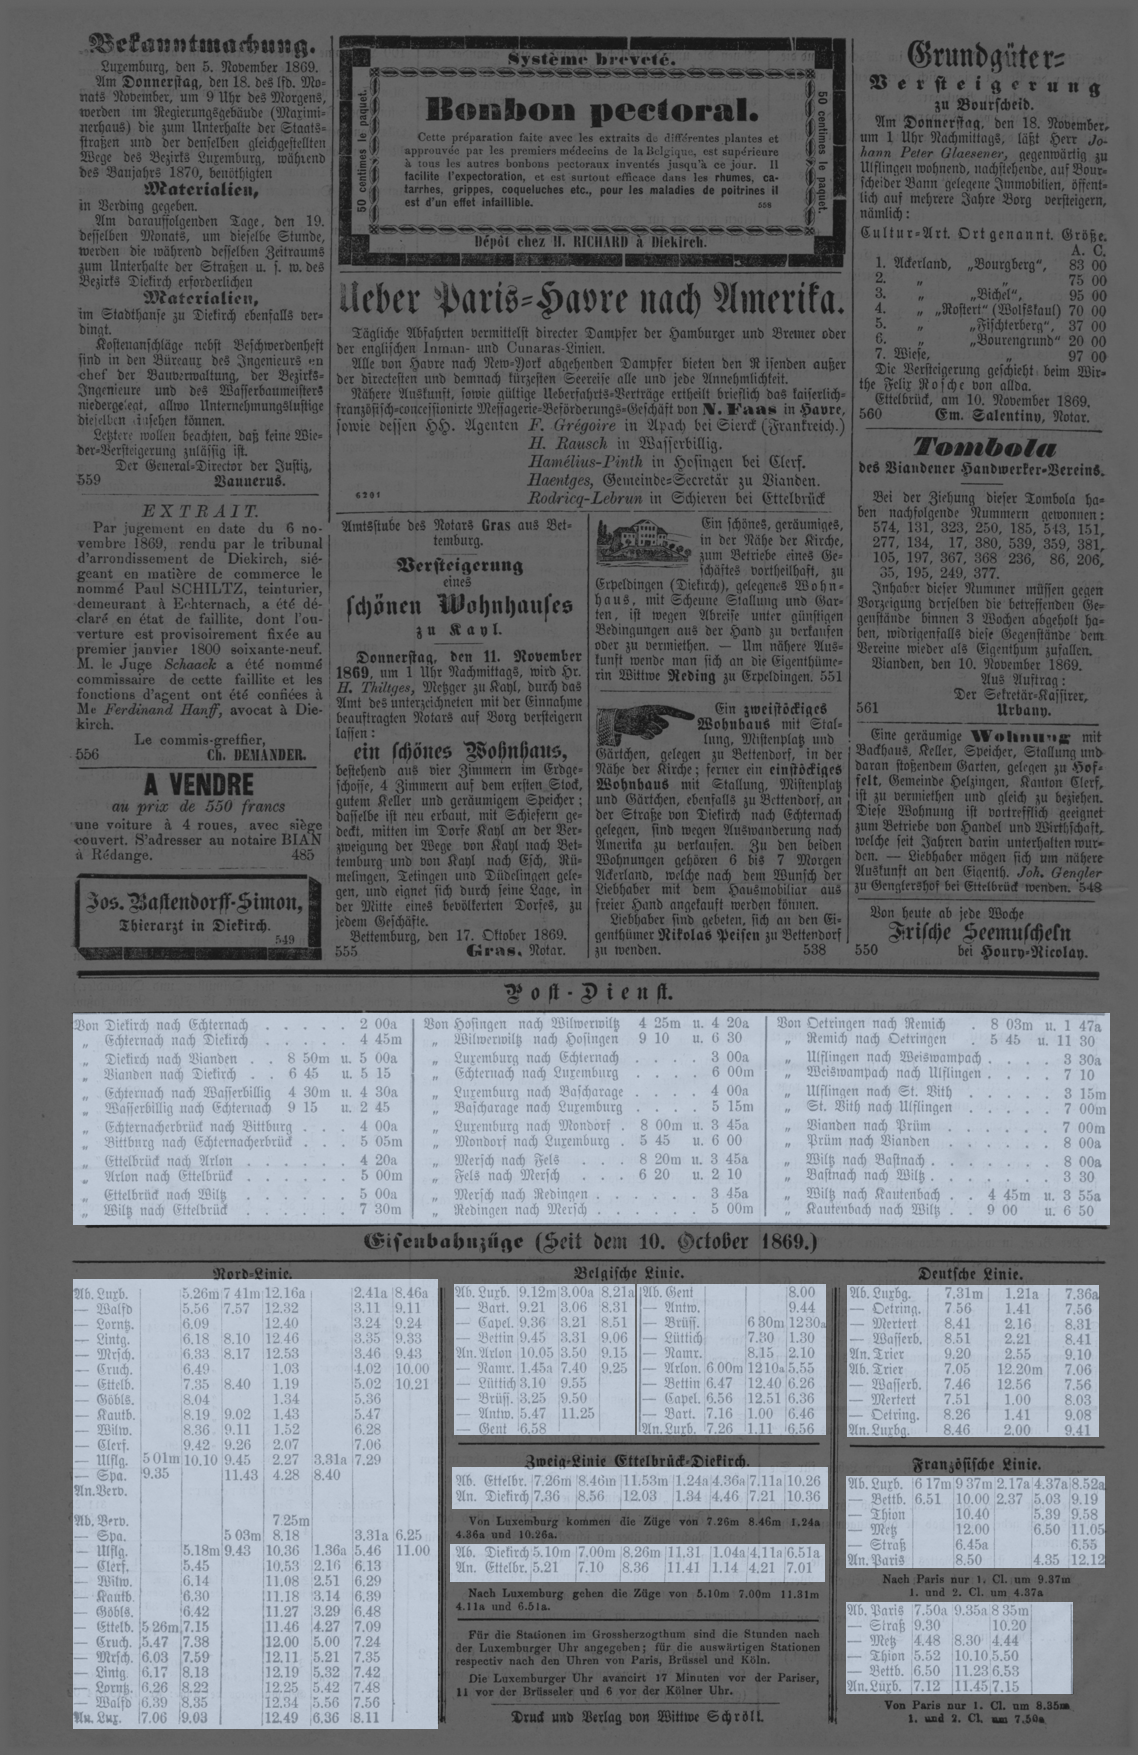
\includegraphics[width=0.30\textwidth]{gt_dhsegment.png}} &
\subfloat[Probability map for tables]{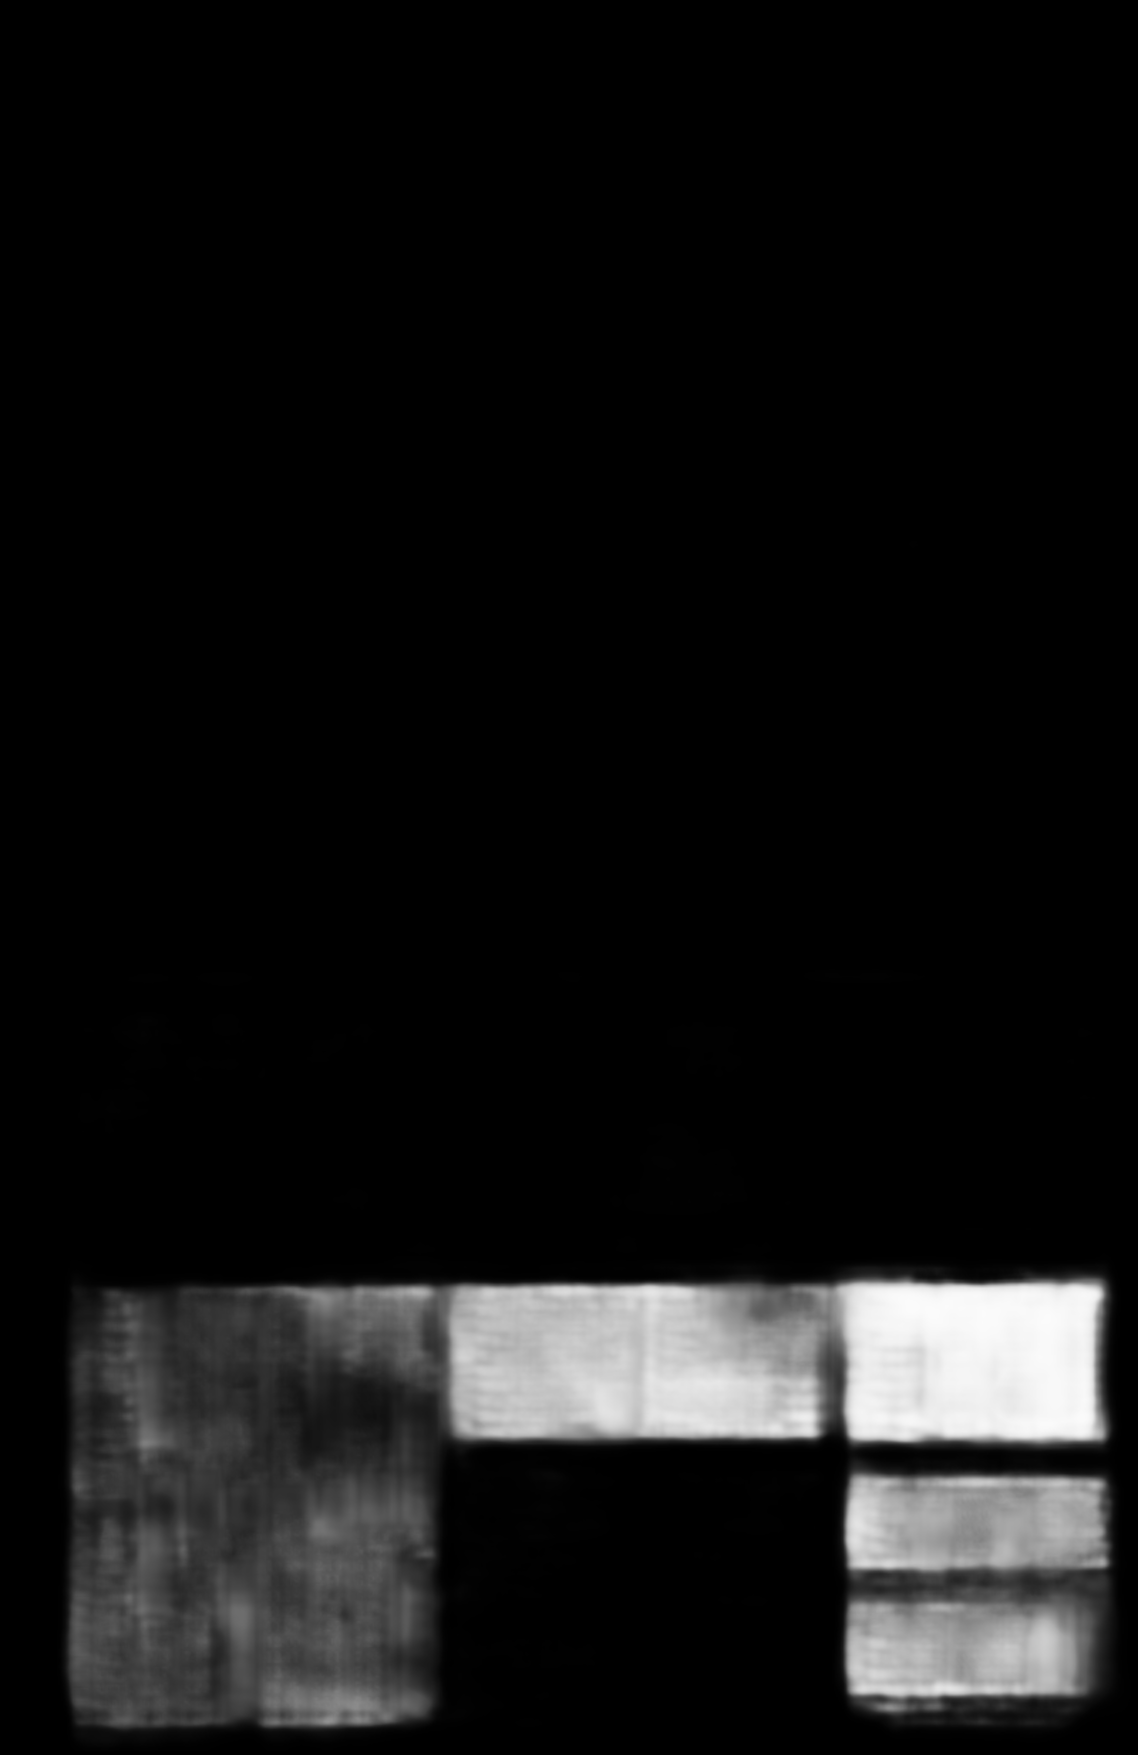
\includegraphics[width=0.30\textwidth]{prob_dhsegment.png}} & 
\subfloat[Prediction map]{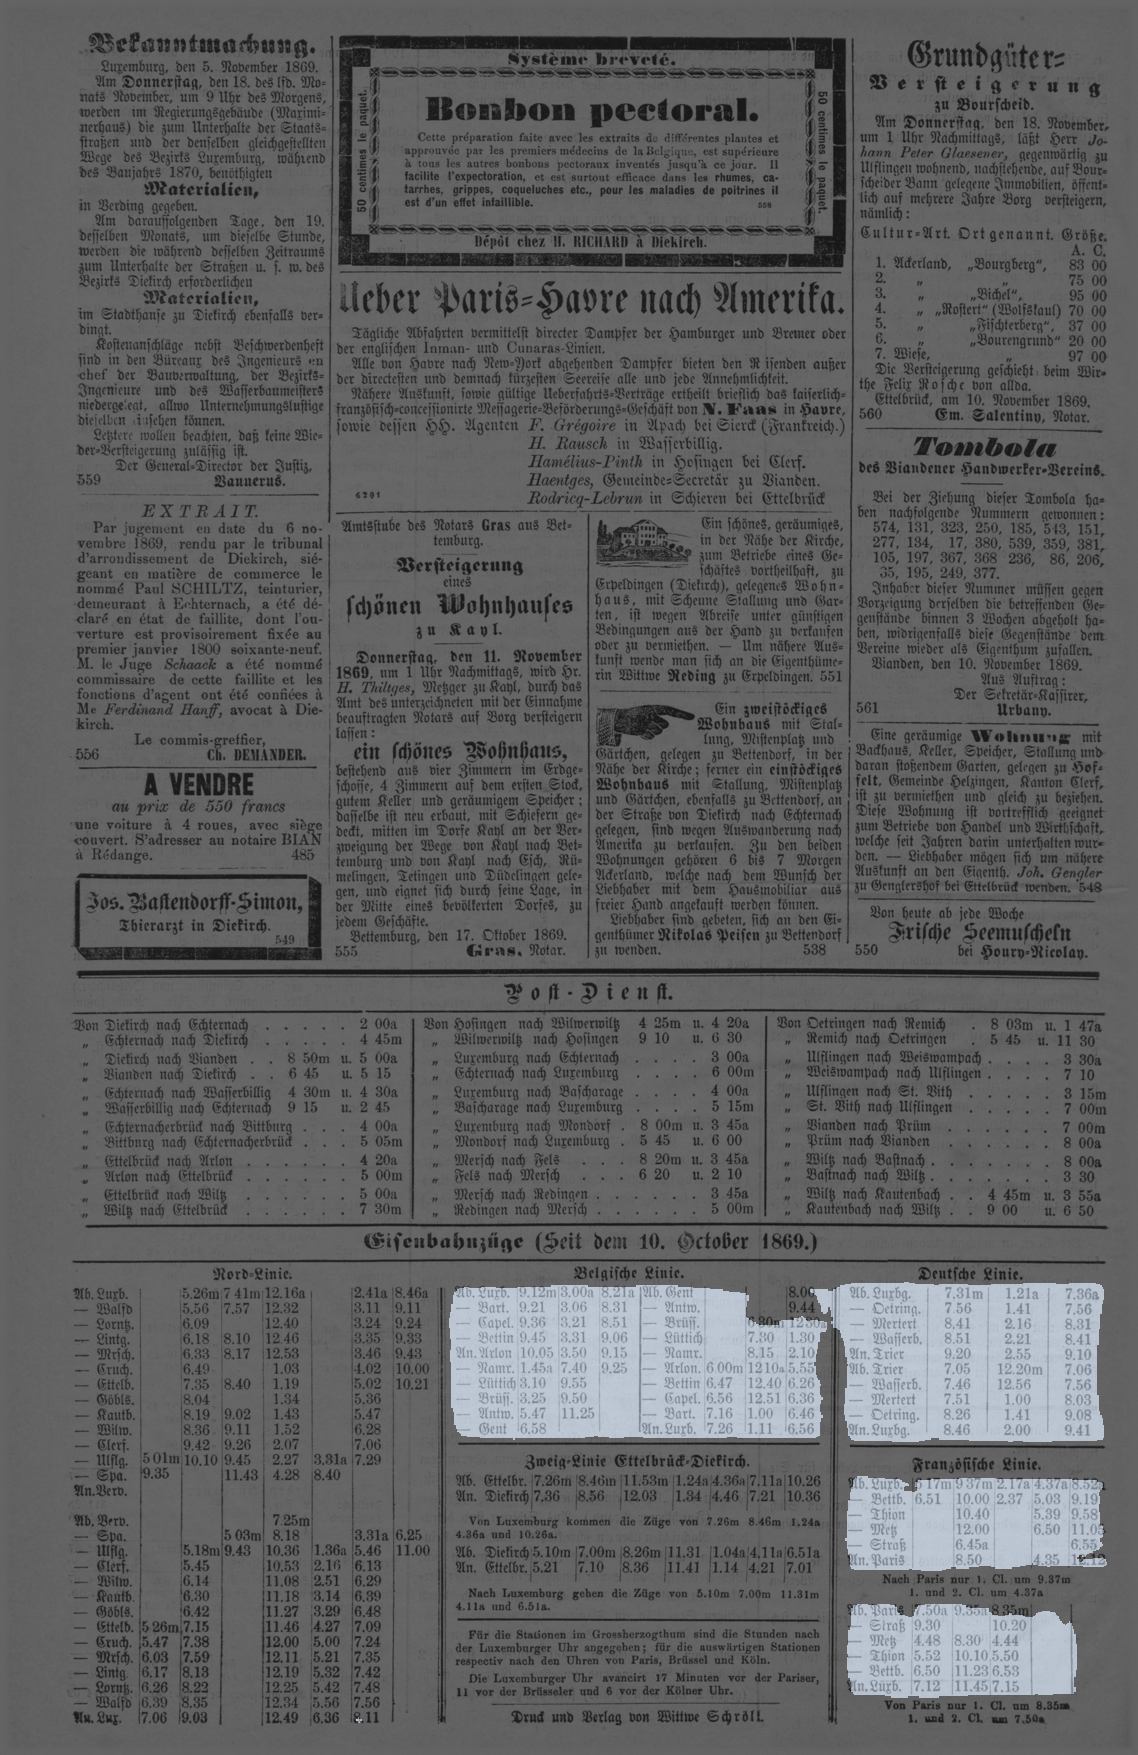
\includegraphics[width=0.30\textwidth]{pred_dhsegment.png}}\\
\end{tabular}
\caption{Inference process of dhSegment.}
\label{inference_dhsegment}
\end{figure}

\subsection{Mask R-CNN}
Mask R-CNN \citep{he_mask_2018} is an object instance image segmentation algorithm, originally developed at Facebook AI Research and commonly used for its versatility, which has shown good results for document image analysis. Built after the Faster R-CNN architecture \citep{ren_faster_2016}, it follows the same two-stage procedure with slight improvements. First, feature maps are generated for the image using a feature extractor network, that is referred as the \textit{backbone}. These are passed through a region proposal network (RPN) that detects regions of interest (RoI). Second, visual features are extracted and pooled from the image feature maps for each RoI using an operation called RoIAlign. RoIAlign ensures that the extracted sub-maps for each RoI have the same dimensions and are not affected by quantization problems induced by dimension changes. The feature sub-maps of each RoI finally pass through the \textit{head} of the backbone and an added branch for mask segmentation. A label, bounding box coordinates and a segmentation mask (at the pixel level) within the bounding box are finally output for each RoI. Note that ResNet models \citep{he_deep_2015} are generally the preferred choice for the backbone, and that its head refers to the final layers used for prediction, which will differ for each model.\\
The implementation of Mask R-CNN used in this project comes from the MMDetection library \citep{chen_mmdetection_2019}, an open-source toolbox for image detection tasks.

\paragraph{Object instance image segmentation}
We recall the definition of object instance image segmentation and complete it according to our specific case. Object instance segmentation consists in detecting clusters of pixels belonging to the same semantic class while identifying each instance of that class separately. It therefore requires fine-grained ground truth annotations, as each table must be distinctly annotated for models to understand they are different instances of the same semantic class. It differs from semantic image segmentation in that regard.\\
When talking about object instance image \textit{detection}, as opposed to object instance image \textit{segmentation}, the goal is only to detect objects (with a bounding box) and not to actually segment them. Because these tasks are so popular, they have their share of conventional formats associated with them for annotations. COCO \citep{lin_microsoft_2014} being one of them, it was used in this project and is briefly described below.

\paragraph{COCO}
Common Objects in Context (COCO) is originally a dataset compiled by Microsoft that contains a large amount of images representing complex scenes of everyday life annotated according to an annotation format they proposed. This format is now widely used for object instance detection tasks and had to be used here in order to feed the data to the MMDetection library. \\
COCO also refers to a series of competitions around image detection tasks\footnote{\url{https://cocodataset.org/\#detection-eval}} in which many metrics have been chosen to compare the performance of models and have become standards in the field. These metrics are explained later in \ref{table_detection_evaluation}.

\paragraph{Model}
The architecture of the Mask R-CNN model used in this project is somewhat similar to that of dhSegment, as the backbone of its convolutional architecture is also a ResNet-50. However, it is also coupled with a Feature Pyramid Network (FPN) \citep{lin_feature_2017} that helps extract better features from the RoI by compiling in a top-down manner the feature maps generated by the backbone. The model was pretrained on the ImageNet dataset for 36 epochs. 

\paragraph{Training}
The training hyper-parameters are detailed later, as they vary from experiment to experiment. However, what remains constant is the use of the mean average precision (mAP) metric (see Section \ref{table_detection_evaluation}), on the segmentation masks, to guide the training of the network. Indeed, the mAP can be computed either based on the segmentation masks of each proposed instance by the model or on their bounding boxes. Since tables are not always rectangular, we force the network to learn on the segmentation masks. Therefore, each evaluation metric reported in this thesis for Mask R-CNN are computed using these. 

\paragraph{Inference}
The model outputs the bounding box coordinates of each of the detected instances, as well as a segmentation mask within these bounding boxes along with a confidence score ranging from 0.05 to 1 for each instance. An example is shown in Figure \ref{example_mask}, where the ground truth of each table instance is shown in blue, and each prediction is shown as a red bounding box and a segmentation mask inside. The confidence score and class of each prediction is marked at its top.

\begin{figure}
\centering
\begin{tabular}{cc}
\subfloat[Ground truths (blue) and object instance predictions (red)\label{example_mask}]{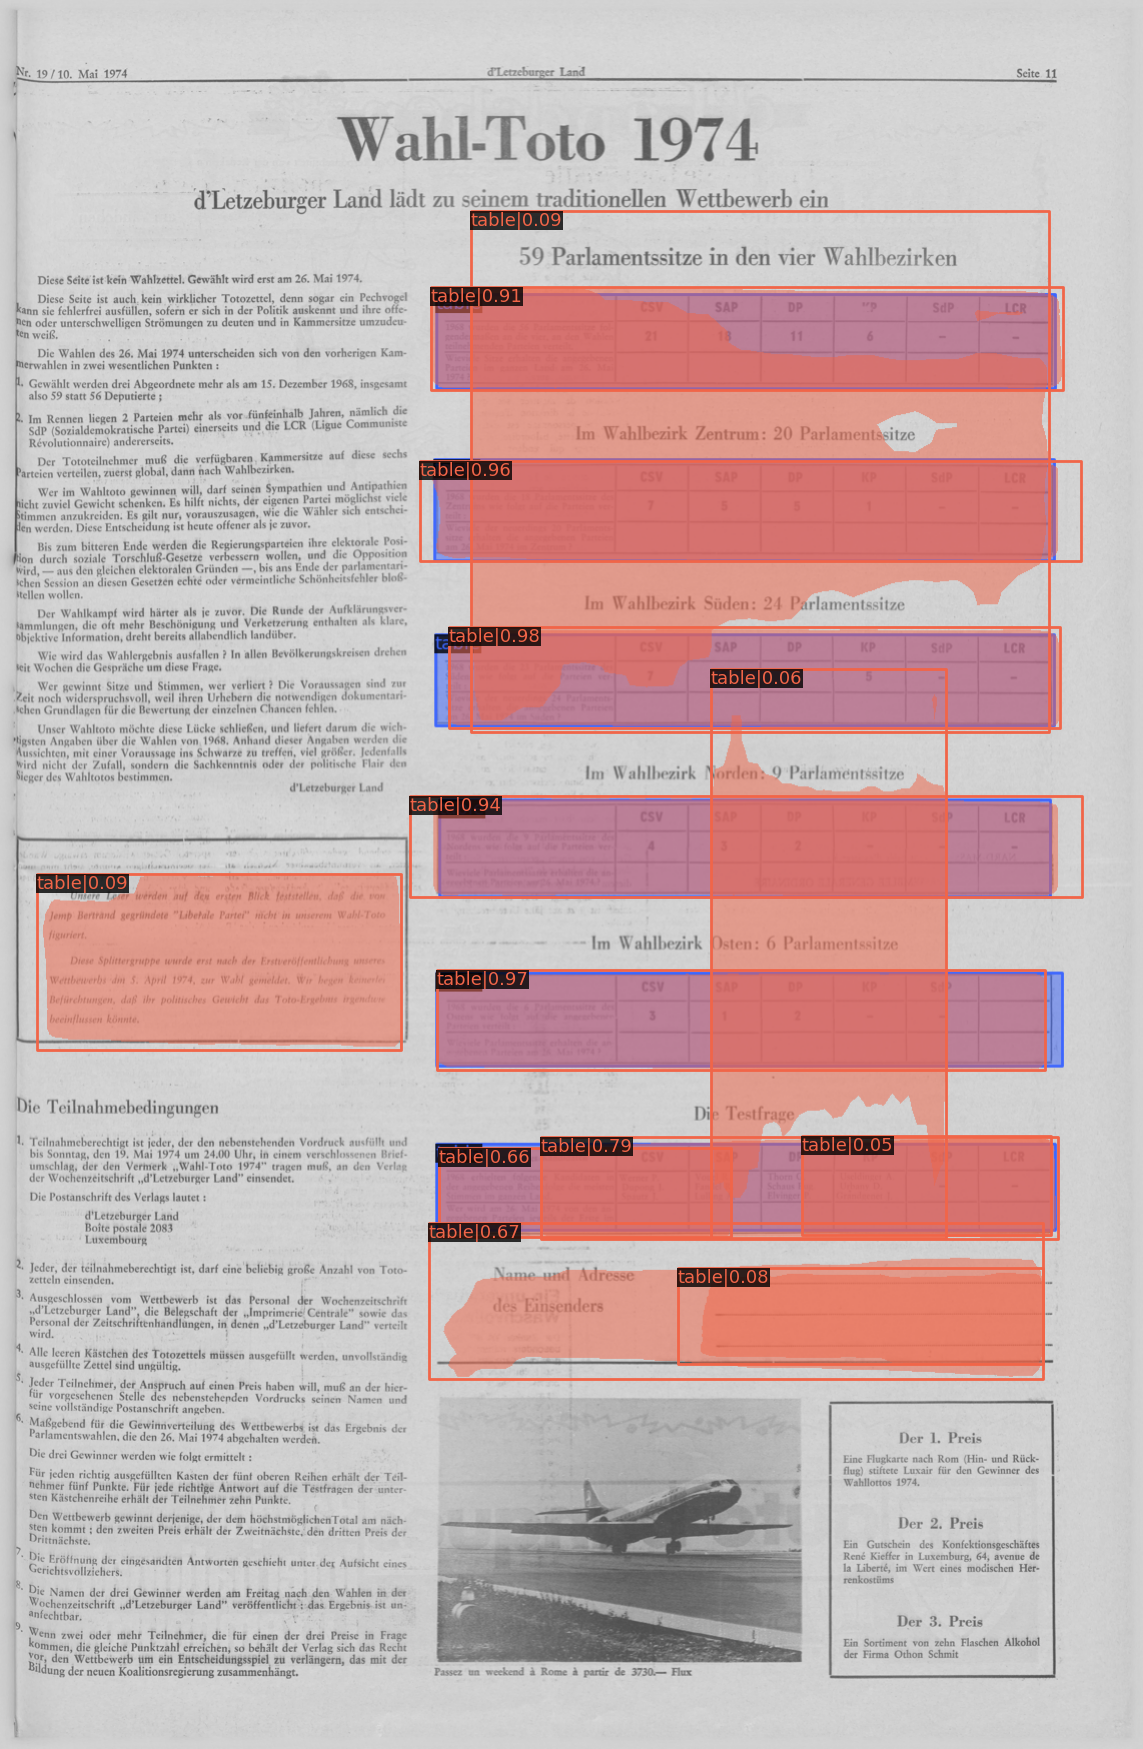
\includegraphics[width=0.45\textwidth]{pred_mask.png}} &
\subfloat[Semantic prediction\label{prediction_mask}]{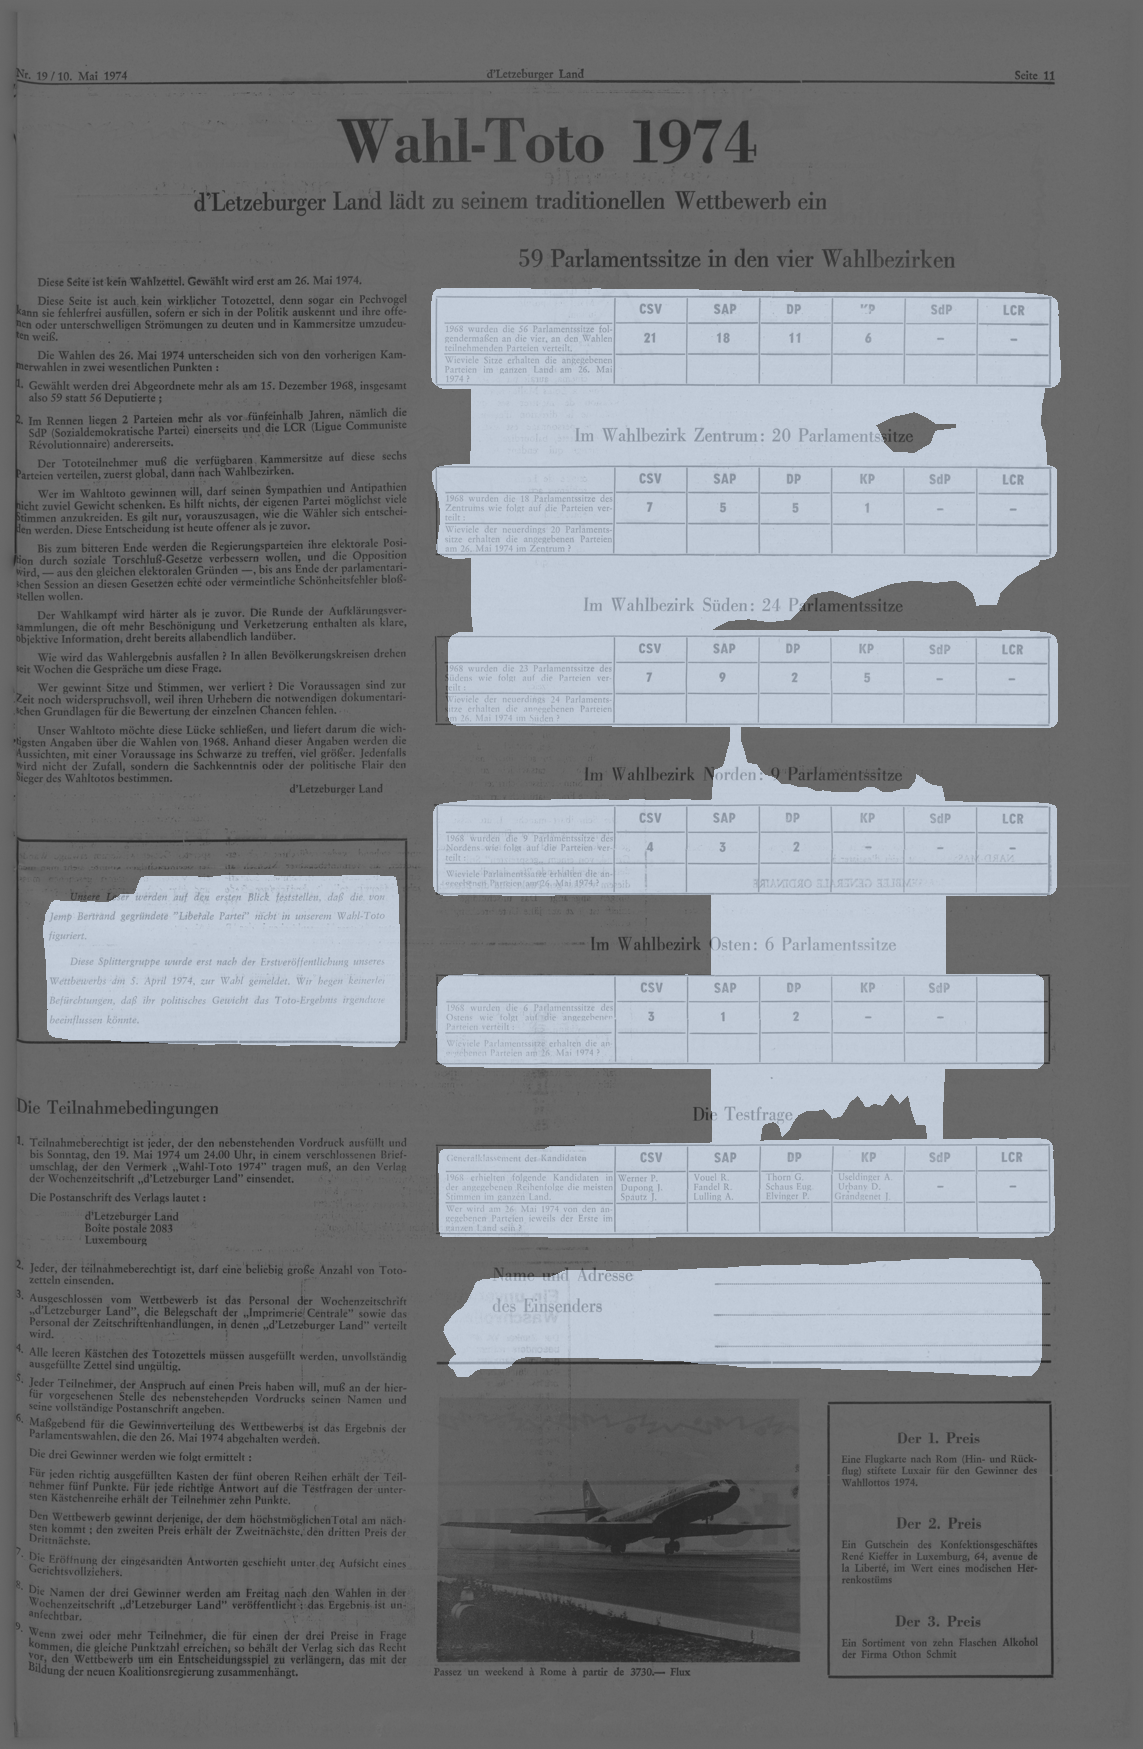
\includegraphics[width=0.45\textwidth]{semantic_mask.png}} \\
\end{tabular}
\caption{Comparison between Mask R-CNN object instance and semantic predictions.}
\label{inference_mask}
\end{figure}

\subsection{Evaluation}
\label{table_detection_evaluation}
Semantic image segmentation and object instance image segmentation are two tasks that each have well-established sets of metrics used to evaluate models. Some of these metrics are presented here, starting with the Intersection over Union (IoU) used for semantic segmentation. Next, the Average Precision (AP), a widely used metric for object instance image segmentation tasks and the primary metric for COCO challenges, is explained. Finally, the relationship between these metrics is explained, as well as a strategy for effectively comparing semantic and object instance segmentation models.

\subsubsection{IoU (Intersection over Union)}
The IoU measures the quality of a predicted segmentation mask by computing its intersection with the corresponding ground truth segmentation mask over their union. Formally, if P is the set of predicted pixels and G the set of pixels belonging to the ground truth, IoU is defined as follows:
\[ IoU(P,G) = \frac{|P \cap G|}{|P \cup G|} \]
Often, this metric is computed for every images and every classes to be detected and then averaged. It is referred to as the mean Intersection over Union (mIoU). If $P$ is the set of all predictions, $G$ is the set of all ground truths, $P_{i,c}$ is the set of pixels predicted for image $i$ and class $c$, $G_{i,c}$ the set of pixels that belongs to the ground truth for image $i$ and class $c$, $I$ is the set of images, $C$ is the set of classes, and $I_{c} = \{i \in I : | P_{i,c} \cup G_{i,c}| > 0\}$, then the mIoU is computed as follows:
\[ mIoU(P,G) =\frac{1}{|C|}\frac{1}{|I|} \sum_{i \in I, c \in C}IoU(P_{i,c}, G_{i,c}) \]
Note that the mIoU can also be computed on a per-class basis in order to assess the quality of a model on each class individually, by having only one class in $C$. \\

\subsubsection{AP (Average Precision)}
\label{ap}
AP corresponds to the area under the Precision-Recall curve.

\paragraph{Precision-Recall curve}
The Precision-Recall curve is a function that maps recall to precision for a given model on a specific class. As a reminder, precision is an empirical evaluation measure of a model's ability to make predictions that match ground truths, while recall is an empirical evaluation measure of a model's ability to predict all ground truths. Formally, if TP stands for the number of true positives, TN for true negatives, FP for false positives and FN for false negatives, they are defined as follows:
\[ \text{Precision} = \frac{TP}{TP + FP} \]
\[ \text{Recall} = \frac{TP}{TP + FN} \]
When computing the precision for a certain recall, predictions are sorted by their confidence level and only the first predictions necessary for the model to reach the given recall are considered in the computation of the precision. Since the range of values the recall can take is finite, values between two consecutive points are interpolated by linking these two points. \\
Different strategies are then taken to compute the area under the curve. Generally, a set of evenly spaced recall levels is determined and precision is computed for these recalls. Since a specific recall may not exist for a given solution, the precision for this specific recall value becomes the maximum precision for every recall values larger than the one considered. When computing the AP for the COCO challenge, the set of considered recalls corresponds to $\{0.01*x : x \in \mathbb{Z}_{[0, 100]} \}$, i.e. a set of 101 evenly spaced recall values. In this project this definition is used when computing the AP. \\
Often, this metric is computed for every classes to be detected and then averaged. It is then referred to as mean Average Precision (mAP), even though sometimes also loosely referred to directly as AP. 

\subsubsection{IoU as a threshold}
The IoU is often used to determine whether a prediction should be considered correct or not. It can then be used in conjunction with more traditional metrics such as precision and recall in image segmentation algorithms. The methods for computing precision and recall for semantic image segmentation algorithms and object instance image segmentation algorithms are similar in their use of the IoU to determine the correctness of a prediction, but differ in the amount of predictions made per image.\\
Semantic image segmentation algorithms produces a single mask per image and per class. To assess the correctness of a solution, the following methodology is used. When the IoU between a prediction and a ground truth is above a threshold $\tau$, the prediction is considered a true positive (TP). When $0 < IoU < \tau$, the prediction is considered as a false positive (FP). When no prediction is made and the union is equal to 0, the prediction is considered a true negative (TN). Finally, when $IoU = 0$ and the size of the ground truth is larger than 0, the prediction is considered a false negative (FN). Therefore, the precision and the recall of a semantic segmentation model can be computed, but works on a page level and therefore it is not possible to know exactly how many tables were detected.\\
Object instance image segmentation algorithms make many predictions per image and per class. In this paradigm, to assess the quality of a solution, a similar methodology is followed. The same logic is followed for TP, FP and FN. However, TNs are not considered as there could be infinitely many instances of bounding boxes that should not be detected on a page. Since TNs are not considered in the computation of precision and recall, it is not an issue. Another important aspect to point out is that when multiple predictions are made for a same ground truth object, only the one with the largest IoU is counted as a TP while the others are counted as FP. \\
With this in mind, it becomes clear that precision and recall must be computed by setting a threshold on the IoU beforehand. Precision is then referred to as Precision at $\tau$ or P@$\tau$, and recall follows the same logic. Note that it is also possible to average a metric over multiple IoU thresholds as well. One may want to average precision over IoU values ranging from $\tau_{start}$ to $\tau_{end}$ with a step of $\tau_{step}$, this would be written as P@$\tau_{start}$:$\tau_{step}$:$\tau_{end}$. The same logic follows for recall. Finally, note that since (m)AP relies on precision, recall and thus on the IoU, it also follows the same notation logic.

\subsubsection{Comparing semantic and object instance image segmentation algorithms}
As explained, semantic image segmentation algorithms and object instance image segmentation algorithms are difficult to compare because the numbers of TPs, FPs, TNs and FNs may largely differ. A simple solution is proposed in this project by interpreting the solution produced by the latter class of algorithms as if it had been output by a semantic image segmentation algorithm. To do so, the segmentation masks of each object instance proposed by the algorithm are considered as if they were the result of a single prediction and are thus merged into a single segmentation mask per image. Thus, it is now possible to compute the mIoU at the page-level as it is the case for semantic image segmentation algorithms. An example can be seen in Figure \ref{prediction_mask}, where the original output of Mask R-CNN seen on the left figure is modified as explained. Note that, as explained earlier, the predictions of Mask R-CNN all have a confidence score, starting from 0.05, associated with them. In the methodology we propose here all predictions with a score greater or equal to 0.05 are considered and turned into a semantic mask.

\section{Table classification}
\label{table_classification}
Table classification, in the context of this thesis, refers to the task of classifying tables found in newspaper pages. More formally, given an image that corresponds to a table segment from a scan of a newspaper page, as well as its OCR (text tokens and their bounding box coordinates), the goal is to classify said table using a given label set. Three models using different combinations of data modalities, including text, layout information and images, were used and compared on this task.

\subsection{RoBERTa}
RoBERTa \citep{liu_roberta_2019} is a language representation model based on BERT \citep{devlin_bert_2019}, which stands for Bidirectional Encoder Representations from Transformers. BERT is based on the encoder part of the Transformer architecture \citep{vaswani_attention_2017}, which used two novel strategies for its pre-training. First, the use of masked language modelling, where words in sentences are randomly masked and the network is asked to guess them. Second, the task of next sentence prediction, where the network must guess whether two given sentences have been written next to each other, was created. In order for the model to be able to handle this latter task, BERT also improves on the input representation by allowing for an arbitrary span of contiguous text. Input sentences, in the context of BERT, can therefore be arbitrarily long and contain multiple sentences or a complete document. These strategies contributed in making BERT a state-of-the-art model for many language understanding tasks. Note there exist two versions of BERT consisting of differently sized Transformers architecture: the BASE model contains 110M parameters, while the LARGE model contains 340M parameters. Still, RoBERTa is able to improve on BERT by revising its pre-training, essentially increasing the amount of data used for training, changing some key hyper-parameters used in the training setup, and by removing the next sentence prediction task. RoBERTa stands for Robustly optimized BERT approach. RoBERTa is thus a standard language representation model that takes only text as input and can classify it when a sentence (in the BERT sense) classification head, i.e. a linear layer, is connected to the end of the network. 

\paragraph{Model}
The model used in this project is actually a multilingual version of RoBERTa dubbed XLM-RoBERTa \citep{conneau_unsupervised_2020}, that was trained on one hundred different languages. It is motivated by the fact that the newspapers used in this project are written in different languages: French, German and Luxembourgish. The BASE version is used for memory reasons, with a maximum sequence length of 512 tokens.\\
The implementation of the model comes from the transformers library \citep{wolf_huggingfaces_2020}, a large online library of pre-trained machine-learning models. 

\paragraph{Training}
The training is done following the default hyper-parameters proposed by the library in its version 4.14.1 The accuracy of the model on its validation set is the metric chosen to guide its training.

\paragraph{Inference}
The network outputs logits for each class and the class with the largest one is chosen as the prediction.

\subsection{LayoutLM}
\label{layoutlm}
LayoutLM \citep{xu_layoutlm_2019} is a model for document image understanding and information extraction tasks that modifies the original BERT architecture by incorporating additional layout and image information. Each word token is concatenated with an embedding of its bounding box coordinates and a visual embedding of the image region given by its coordinates. In addition to this, a visual embedding of the entire document image is also concatenated. These visual embeddings are produced by Faster R-CNN \citep{ren_faster_2016}.\\
Although this model can use the visual modality, it was not used in this project. In the original paper, this modality was not used during pre-training and was to be used only for fine-tuning. But a second version of the model called LayoutLMv2 \citep{xu_layoutlmv2_2021} was introduced later and used it during pre-training. This new model is therefore better adapted to evaluate the added value of this modality: this model is introduced afterwards in \ref{layoutxlm}. 

\paragraph{Model}
LayoutLM BASE model was used, which is built over BERT BASE model, and is therefore of similar size. Input sequences must be of length 512. The implementation of LayoutLM also comes from the transformers library; note that it lacks a straight-forward way to make use of the visual data.

\paragraph{Training}
The training is done following the default hyper-parameters proposed by the library in its version 4.14.1 The accuracy of the model on its validation set is the metric chosen to guide its training.

\paragraph{Inference}
Trivially, the class with the largest logit is chosen as the prediction.

\subsection{LayoutXLM}
\label{layoutxlm}
LayoutXLM \citep{xu_layoutxlm_2021} is a multilingual extension of LayoutLMv2 \citep{xu_layoutlmv2_2021} trained on 53 languages; the latter is an improved version of the aforementioned LayoutLM where the only difference is the use of the visual modality during its pre-training making it more efficient. 

\paragraph{Model}
LayoutXLM BASE model was used, which is built over BERT BASE model, and is therefore of similar size. It expects input sequences of length 512. The implementation of LayoutXLM also comes from the transformers library.

\paragraph{Training}
Unlike the training of LayoutLM, the visual modality was used when fine-tuning this model. The training is performed following the default hyper-parameters proposed by the library in its version 4.14.1. The accuracy of the model on its validation set is the metric chosen to guide its learning.

\paragraph{Inference}
The class with the largest logit is chosen as the prediction.

\subsection{Evaluation}
\label{table_classification_evaluation}
When it comes to evaluating the quality of a classifier, precision and recall are commonly used and have already been defined in \ref{ap}. Accuracy is also often used, it measures the proportion of correct predictions made by a model and can be defined as follows:
\[ \text{Accuracy}=\frac{TP + TN}{TP + TN + FP + FN}\]
Finally, another important metric is the F1-score, which can be defined as the harmonic mean of the precision and recall. More formally,
\[ \text{F1-score}=2*\frac{Precision * Recall}{Precision + Recall}\]
Since the problem at hands requires classifying objects into several classes, which may be largely unbalanced and thus strongly bias the above mentioned metrics, it is interesting to run these metrics separately on each class. Another tool to better visualize the results obtained is the confusion matrix which integrates the number of good and bad predictions for each class and allows to easily see which classes are confused by the classifier.